\documentclass[12pt, twoside]{article}
\usepackage[letterpaper, margin=1in, headsep=0.5in]{geometry}
\usepackage[english]{babel}
\usepackage[utf8]{inputenc}
\usepackage{amsmath}
\usepackage{amsfonts}
\usepackage{amssymb}
\usepackage{tikz}
\usepackage{yhmath}
\usetikzlibrary{quotes, angles}

\usepackage{graphicx}
\usepackage{enumitem}
\usepackage{multicol}

\usepackage{fancyhdr}
\pagestyle{fancy}
\fancyhf{}
\renewcommand{\headrulewidth}{0pt} % disable the underline of the header

\fancyhead[RE]{\thepage}
\fancyhead[RO]{\thepage \\ Name: \hspace{3cm}}
\fancyhead[L]{BECA / Dr. Huson / 10th Grade Geometry\\* 9 May 2019}

\begin{document}
\subsubsection*{10.11 Do Now: Algebra, slope, \& review}
 \begin{enumerate}

  \item   Solve for the value of $x$.\\[0.5cm]
  $\frac{1}{5}(2x+3)=1$ \vspace{3cm}

  \item Given $f(x)=\frac{1}{4} x+4$. Solve for $x$ such that for $f(x)=6$. \vspace{3.5cm}
  \item Given $g(x)=3x^2-7x+5$. Simplify $g(0)$. \vspace{2cm}
  \item Given $f(x)=5x-22$. Solve for $x$ such that for $f(x)=3$. \vspace{3.5cm}
  \item Given $h(x)=x^2+6x+5$. Solve $h(x)=0$. \vspace{3cm}

\newpage
  \item A translation maps $A(3,5) \rightarrow A'(-2,7)$. What is the image of $B(-4,1)$ under the same translation?  \vspace{1.5cm}

  \item The line $l$ has the equation $y=-\frac{3}{5}x+4$. To each line below, circle whether $l$ is parallel, perpendicular, or neither.
    \begin{enumerate}
      \item parallel \quad perpendicular \quad neither \qquad $y=\frac{3}{5}x-2$
      \vspace{0.5cm}
      \item parallel \quad perpendicular \quad neither \qquad $3x-5y=-15$
      \vspace{2.5cm}
    \end{enumerate}

  \item Simplify each expression. (Leave it in radical form if necessary, not a decimal.)
    \begin{enumerate}
      \begin{multicols}{2}
      \item   $\sqrt{20}$ \vspace{1.25cm}
      \item   $\sqrt{\frac{16}{49}}$ \vspace{1.25cm}
      \end{multicols}
    \end{enumerate} \vspace{2cm}


  \item Given $m\angle R=40$ and $m\angle U=80$. Find $m\angle UST$.\\[1cm]
  \begin{tikzpicture}
   %\draw [->, thick] (0,0)--(5,5);
   \draw [<-, thick] (8,0)--(0,0)--(3,3)--(4.5,0);
   \draw [fill] (0,0) circle [radius=0.05] node[below]{$R$};
   \draw [fill] (4.5,0) circle [radius=0.05] node[below]{$S$};
   \draw [fill] (3,3) circle [radius=0.05] node[right]{$U$};
   \draw [fill] (7,0) circle [radius=0.05] node[below]{$T$};
 \end{tikzpicture} \vspace{1cm}

  \item Write down the center and radius of each circle.
   \begin{enumerate}
     \begin{multicols}{2}
     \item   $(x-1)^2+(y+3)^2=81$ \vspace{2.5cm}
     \item   $x^2+y^2=49$ \vspace{2.5cm}
     \end{multicols}
   \end{enumerate} \vspace{2cm}

\newpage
  \item In the diagram below, $\overline{AC}$ has endpoints with coordinates $A(-4, 5)$ and $C(5, 2)$.
   \begin{center} %4 quadrant regents grid
     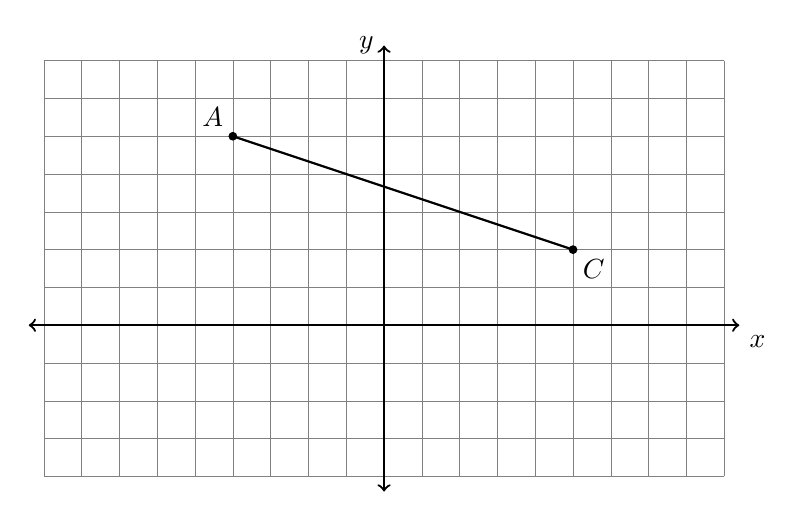
\begin{tikzpicture}[scale=.48]
       \draw [help lines] (-9,-4) grid (9,7);
       \draw [thick, <->] (-9.4,0) -- (9.4,0) node [below right] {$x$};
       \draw [thick, <->] (0,-4.4)--(0,7.4) node [left] {$y$};
       \draw [thick] (-4, 5)--(5, 2);
       \draw [fill] (-4, 5) circle [radius=0.1] node[above left] {$A$};
       \draw [fill] (5, 2) circle [radius=0.1] node[below right] {$C$};
     \end{tikzpicture}
   \end{center}
   If $B$ is a point on $\overline{AC}$ and $AB {:} BC = 1{:}2$,  what  are  the coordinates of $B$? \vspace{4cm}

  \item Triangle $ABC$ is dilated with a scale factor of $k$ centered at $A$, yielding $\triangle ADE$, as shown. Given $AB=9$, $BC=12$, $AC=15$, and $DE=16$. \\[0.25cm] Find $BD$, $AE$, and $k$ (the scale factor).\\[0.25cm]
     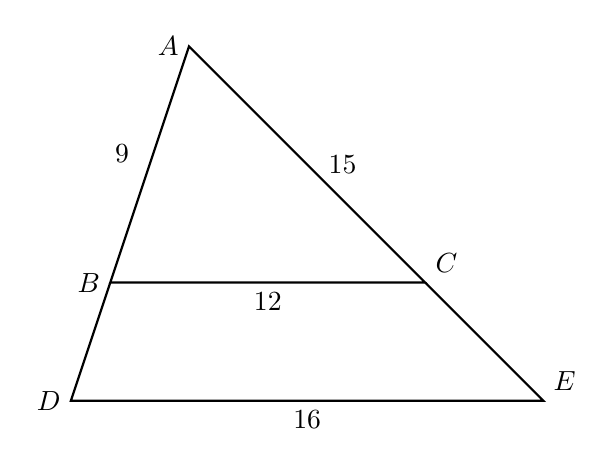
\begin{tikzpicture}[scale=0.5]
       \draw [thick]
       (0,0)node[left]{$B$}--
       (8,0)node[above right]{$C$}--
       (2,6)node[left]{$A$}--cycle;
       \draw [thick]
       (0,0)--
       (-1,-3)node[left]{$D$}--
       (11,-3)node[above right]{$E$}--(8,0);
       \node at (4,0)[below]{$12$};
       \node at (5.3, 3)[right]{$15$};
       \node at (0.3, 2.8)[above]{$9$};
       \node at (5,-3)[below]{$16$};
     \end{tikzpicture}
  \vspace{2cm}

\newpage
  \item What is the smallest non-zero angle of rotation about its center that would map the octagon onto itself? \vspace{0.25cm}
  \begin{center}
    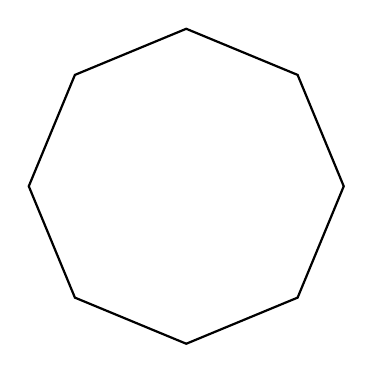
\begin{tikzpicture}%[scale=.48]
      \draw [thick]
      (0:2)--
      (45:2)--
      (90:2)--
      (135:2)--
      (180:2)--
      (225:2)--
      (270:2)--
      (315:2)--cycle;
    \end{tikzpicture}
  \end{center} \vspace{2cm}

  \item What transformation maps $\triangle ABC$ onto $\triangle DEF$, shown below? Fully specify the transformation.
    \begin{center}
      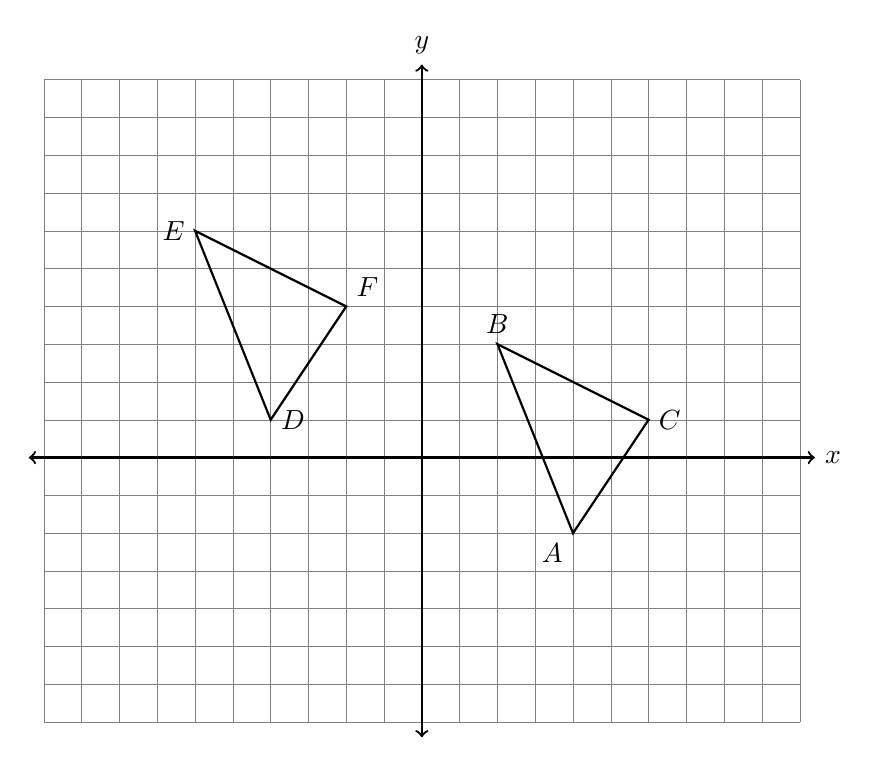
\begin{tikzpicture}[scale=.48]
        \draw [help lines] (-10,-7) grid (10,10);
        \draw [thick, <->] (-10.4,0) -- (10.4,0) node [right] {$x$};
        \draw [thick, <->] (0,-7.4)--(0,10.4) node [above] {$y$};
        \draw [thick]
          (4,-2) node[below left] {$A$}--
          (2,3) node[above] {$B$}--
          (6,1) node[right] {$C$}--cycle;
        \draw [thick]
          (-4,1) node[right] {$D$}--
          (-6,6) node[left] {$E$}--
          (-2,4) node[above right] {$F$}--cycle;
      \end{tikzpicture}
    \end{center}



\end{enumerate}
\end{document}
